 ------------------------------------------------------------------------------
% Chapter 5
% ------------------------------------------------------------------------------
\chapter{AI} % enter the name of the chapter here
\section{Retrieval augmented generation (RAG)} % enter the name of the section here
Retrieval augmented generation (RAG) is a natural language processing (NLP) technique that combines the strengths of both retrieval- and generative-based artificial intelligence (AI) models
\begin{figure}[h]
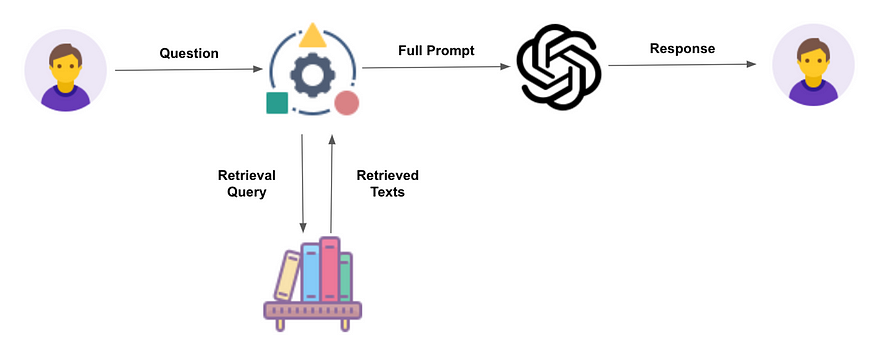
\includegraphics[width=\columnwidth]{rag}
\centering
\end{figure}
\subsection*{why?}
RAG allows the LLM to present accurate information with source attribution
\subsection{Selecting Documents} %enter the name of the subsection here
First we have select an infromative documents to make the bot therapiest more informative and take the right decision towards the correct and scientific response towards the solution.
so we collected alot of arabic base and translated books and documents from scholar we need to collect alot of information so we made a web scraper to take inputs and search in google scholar and get back the top articles and books in pdf to store them for the next step to use them in the rag system to cover alot of points in the theraptic direction
\subsection{Chunking} 
Dividing a large text corpus into smaller, manageable pieces or segments. Each chunk acts as a standalone unit of information that can be individually indexed and retrieved.
\begin{figure}[h]
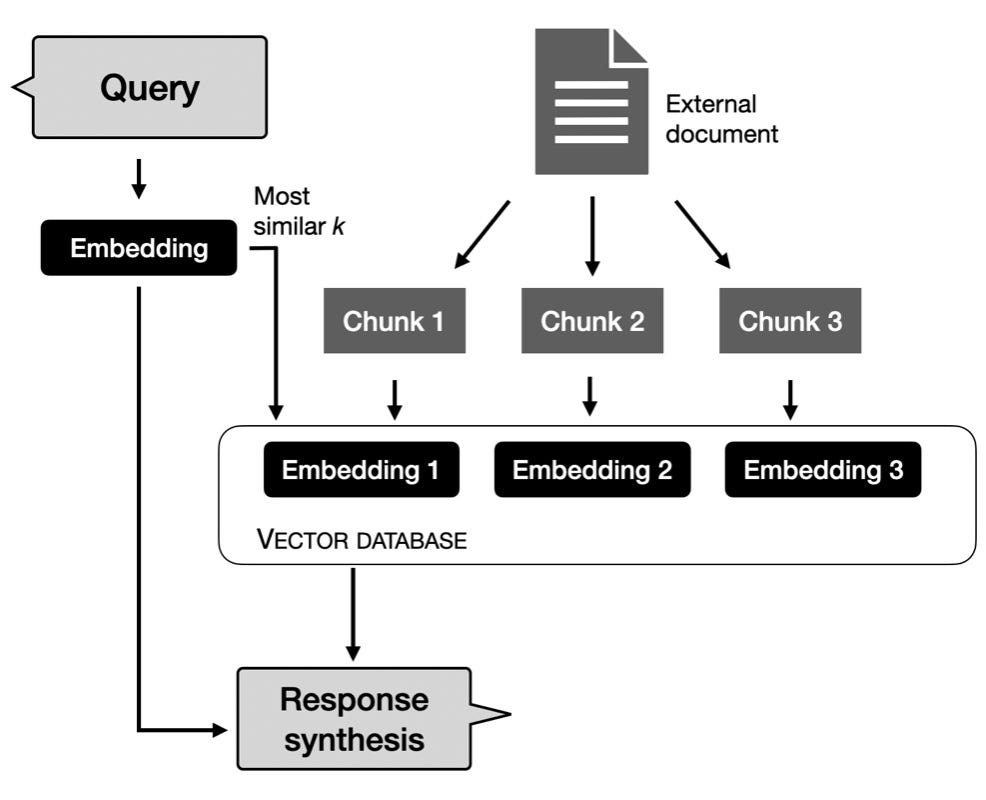
\includegraphics[width=\columnwidth]{chunking}
\caption{showing the chunking process and adding the chunks to the query}
\centering
\end{figure}

\section*{Chunking Methods}

We considered several chunking methods for processing our PDF text:

\begin{itemize}
    \item Fixed Size Chunking
    \item Recursive Chunking
    \item Document Specific Chunking
    \item Semantic Chunking
    \item Agentic Chunking
\end{itemize}



\section*{Why Semantic Chunking?}

Semantic chunking offers the following advantages:
\begin{itemize}
    \item Fast
    \item Efficient
    \item Accurate
\end{itemize}
Therefore, we chose semantic chunking over the other methods.

\subsection{Similarity Search} 
Similarity Search is the way of RAG to get the targeted related part of the pdfs or chunks to embed the information that is related to the current input in the prompt and get more accurate informative results
\begin{figure}[h]
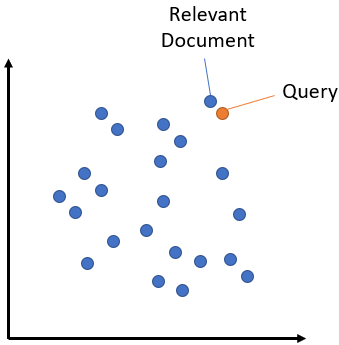
\includegraphics[width=\columnwidth]{simisearch}
\caption{showing the chunking process and adding the chunks to the query}
\centering
\end{figure}

\subsection{embedding in the prompt}
And after we retrived the chuncks we embed it in the prompt to be passed to the tokenizer and then to the model after that to get the best accurate result to get the knowledge of the therapist embedded in the tuned model to be your friend therapist



\subsection{Introduction}
To enhance our understanding of emotions in text, we decided to create a classification model that takes a user's input message and predicts the corresponding emotion. This model can be particularly useful in sentiment analysis and mental health monitoring. By accurately detecting emotions, we can improve user interactions and provide more empathetic responses.

\begin{figure}[h]
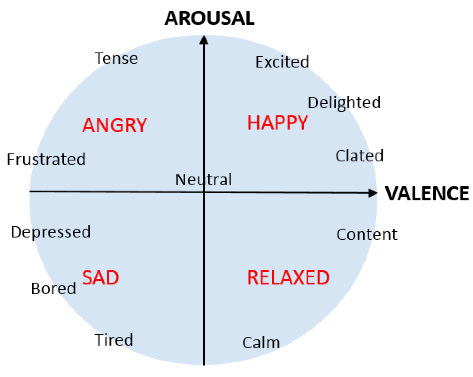
\includegraphics[width=\columnwidth]{emo1}
\centering
\end{figure}

\subsection{Selecting Dataset}
We chose an Arabic dataset named {arabic-empathetic-conversations} for emotion classification. This dataset consists of conversations where each conversation is labeled with an emotion. The dataset has 36,628 rows and 30 unique emotions, organized into three columns: {emotion}, \textit{context}, and \textit{response}. This rich dataset provides a comprehensive basis for training our emotion detection model.

\subsection{Preprocessing}
To prepare the dataset for training, we performed several preprocessing steps:

\begin{figure}[h]
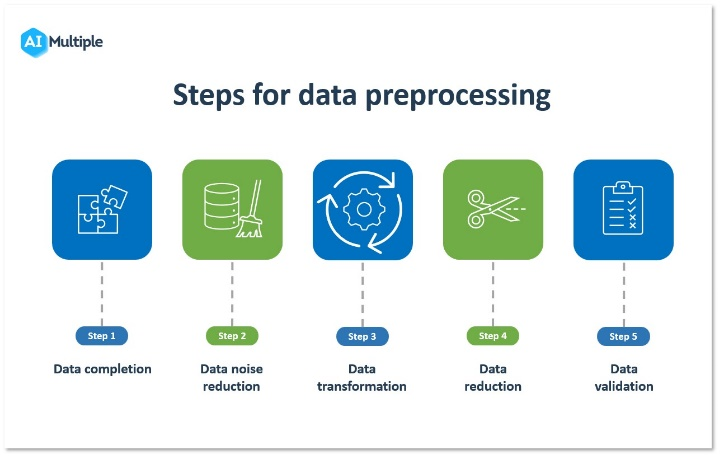
\includegraphics[width=\columnwidth]{emo2}
\centering
\end{figure}
\begin{enumerate}
    \item \textbf{Emotion Selection}: We selected a subset of unique emotions, reducing the dataset size to 5,820 rows. This step helps to focus on the most relevant emotions and reduces the complexity of the model.
    \item \textbf{Combining Text}: We concatenated the {context} and {response} columns into a single column named \textit{text} to represent the entire conversation. This ensures that the model has all the necessary information in a single input field.
    \item \textbf{Label Encoding}: We converted the emotion labels into numerical indices using a mapping dictionary ({lbl2idx}). For example, the mapping looked like this: \{‘joyful’: 0, ‘sad’: 1, ‘lonely’: 2, ‘anxious’: 3, ‘content’: 4\}. This numerical encoding is essential for training machine learning models.
    \item \textbf{Imbalancing}: To address class imbalance, we used the {oversample\_data} function. This function oversamples the minority classes by randomly duplicating samples until each class has the same number of samples as the majority class. This helps prevent the model from being biased towards the majority class during training. The function utilizes the {resample} function from the \textit{sklearn.utils} module.
\end{enumerate}

\section{Data Splitting}
We split the dataset into training, validation, and test sets as follows:

\begin{figure}[h]
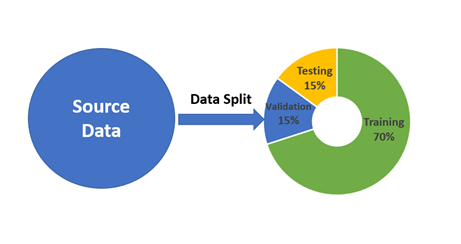
\includegraphics[width=\columnwidth]{emo3}
\centering
\end{figure}
\begin{enumerate}
    \item \textbf{Initial Split}: We divided the dataset into training (70\%) and temporary data (30\%) to ensure that the model has enough data to learn from while reserving a portion for testing.
    \item \textbf{Second Split}: We split the temporary data into equal parts for testing and validation (50\% each) to fine-tune the model and evaluate its performance.
\end{enumerate}

The final split sizes were:
\begin{itemize}
    \item Training: 4,074 rows
    \item Validation: 873 rows
    \item Testing: 873 rows
\end{itemize}

This splitting strategy ensures that the model is tested on unseen data, providing a realistic measure of its performance.

\section{Selecting Model}
We chose the BERT model for our classification task, specifically the {aubmindlab/bert-base-arabertv02-twitter} model. BERT (Bidirectional Encoder Representations from Transformers) models are known for their effectiveness in various NLP tasks, including text classification. BERT's ability to understand context from both directions in a sentence makes it particularly powerful for understanding nuanced emotions.

\section{Fine-Tuning}
\begin{enumerate}
    \item \textbf{Model Loading}: We used the {AutoModelForSequenceClassification} class from Huggingface, which helps in loading pre-trained models suitable for sequence classification tasks. We specified the number of labels in our dataset during this step. This class automatically adds a classification head to the model, making it ready for our task.
    \item \textbf{Tokenization}: We used the BERT tokenizer to process the text data. This involved trimming the text to a certain length and adding padding where necessary to ensure uniform input sizes. We also created a custom dataset class to store the tokenized texts and their labels, streamlining the data loading process for training.
\end{enumerate}

\section{Training}
During the training phase, we fine-tuned the BERT model on our preprocessed dataset.
\begin{enumerate}
    \item \textbf{Training Arguments}: We defined various training arguments. These arguments specify where to save the results, how many times to go through the training data, and the number of samples to use in each batch during training and evaluation. They also determine how to adjust the learning rate at the beginning and the strength of weight decay to avoid overfitting. Additionally, the arguments define how often to log and evaluate the model, which in this case is once every epoch.
    \item \textbf{Trainer Class}: We specified the model to be trained in our trainer class and provided the training arguments defined earlier. It also includes the datasets for training and evaluation and a function to calculate performance metrics. This configuration ensures that the model is trained and evaluated with the specified settings, allowing for a structured and efficient training process.
\end{enumerate}

\section{Result}
After fine-tuning the model on our dataset, we evaluated its performance using the validation and test sets. The results demonstrated the model's ability to accurately classify the emotions associated with the given text inputs. Key performance metrics such as accuracy, precision, recall, and F1-score were used to assess the model's effectiveness.

By following these steps, we successfully developed an emotion classification model that can predict emotions from Arabic text inputs. This model can be further refined and applied to various practical applications to understand and respond to human emotions more effectively. Future work could include expanding the dataset, incorporating additional features, and exploring other advanced models to further enhance performance.

\section{LoRA and Q-LoRA}

\section{LoRA}
LoRA (Low-Rank Adaptation) is a technique to fine-tune large language models efficiently by injecting trainable low-rank matrices into each layer of the transformer architecture. This approach reduces the number of parameters that need to be updated during training, making it computationally efficient and cost-effective, especially for tasks requiring adaptation to specific domains or languages.

\section{Q-LoRA}
QLoRA (Quantized Low-Rank Adaptation) builds on LoRA by incorporating quantization techniques. Quantization involves representing model parameters with fewer bits, reducing memory and computational requirements. This saves memory and makes the model run faster, especially on devices with less power.

\begin{figure}[h]
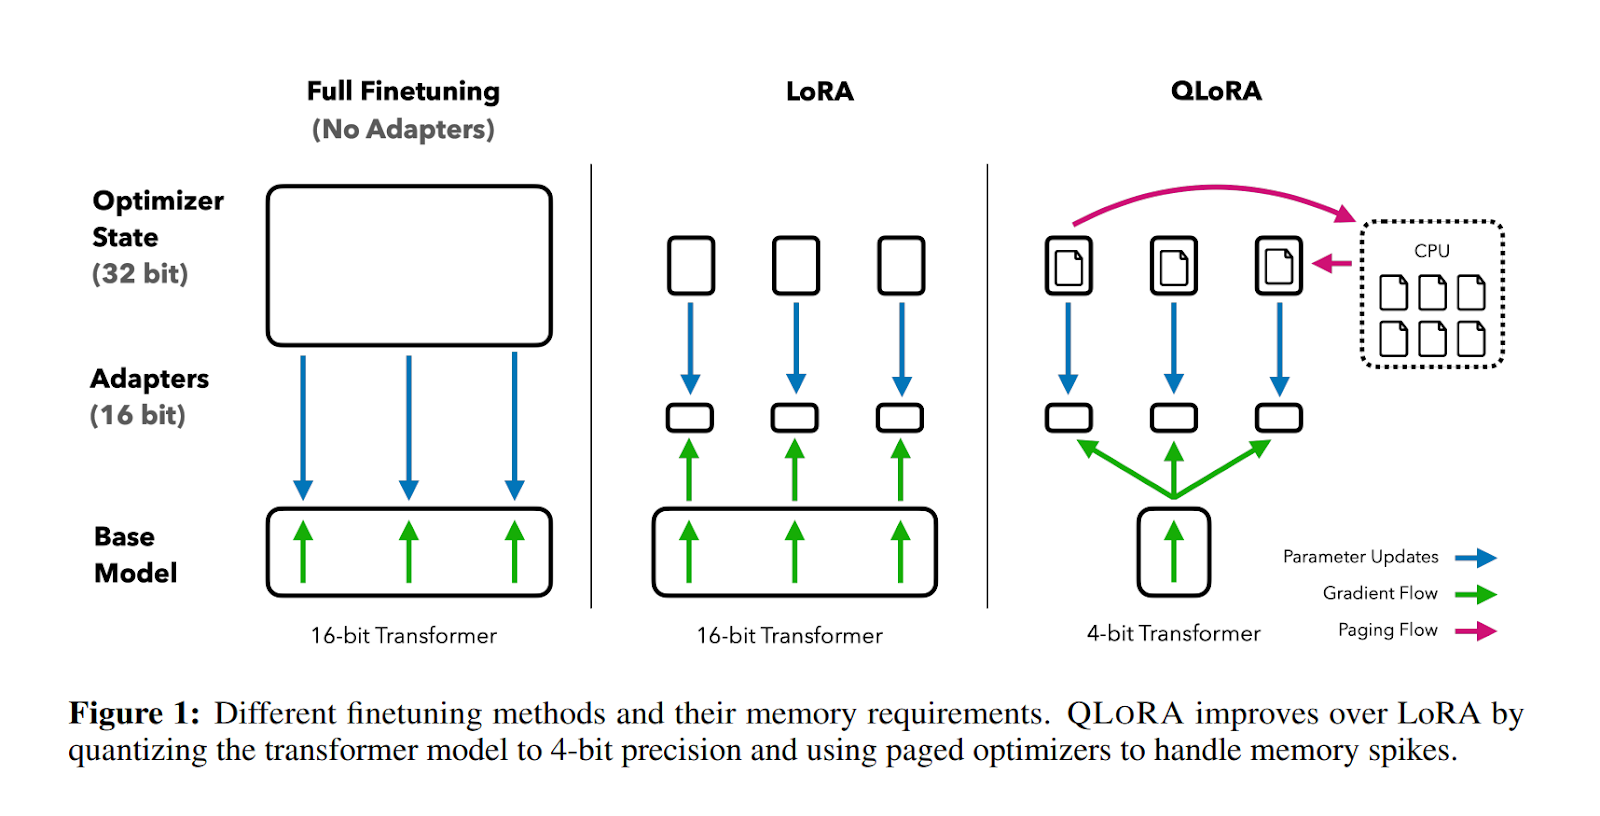
\includegraphics[width=\columnwidth]{emo4}
\centering
\end{figure}
\section{GPU Usage}

\section{Without Q-LoRA}
When we train our model on a GPU without using QLoRA, we use the full precision of the model's parameters.
\begin{enumerate}
    \item \textbf{Full Precision Training}: The model uses 16-bit or 32-bit floating point numbers to represent its parameters. This provides high accuracy but requires more memory and computational power.
    \item \textbf{Memory Usage}: Full precision training uses a lot of GPU memory. For large models, this can quickly fill up the available memory, limiting the batch size and the number of layers we can train simultaneously.
    \item \textbf{Speed}: Training is fast compared to a CPU, but the high memory usage can sometimes slow down the training process if the GPU memory becomes a bottleneck.
    \item \textbf{Results}: Full precision training can lead to slightly better results because there’s no loss of detail in the model’s parameters. However, the difference might not be significant enough to justify the extra resource use.
\end{enumerate}

\section{With Q-LoRA}
When we use QLoRA (Quantized Low-Rank Adaptation) on a GPU, we optimize the training process by reducing the precision of the model’s parameters.
\begin{enumerate}
    \item \textbf{Quantization}: We use 4-bit quantization for the model’s parameters. This means we represent each parameter with fewer bits, drastically reducing the memory footprint.
    \item \textbf{Memory Usage}: With 4-bit quantization, the memory usage drops significantly. This allows us to train larger models or use larger batch sizes without running into memory limitations.
    \item \textbf{Speed}: Training becomes faster because the model is smaller and requires fewer computations. The GPU can process more data in parallel, leading to quicker training times.
    \item \textbf{Results}: While there’s a slight reduction in precision, QLoRA is designed to maintain high performance. The trade-off between memory efficiency and model accuracy is minimal, and in many cases, the results are comparable to full precision training.
\end{enumerate}

\section{Simple Example}
Training a large language model on a GPU without QLoRA might take 10 hours and use up 90\% of the GPU's memory, while training the same model on a GPU with QLoRA might take only 6 hours and use just 50\% of the GPU's memory.

\section{Training Process}
When we train the model, we follow these steps:
\begin{enumerate}
    \item \textbf{Set Up Quantization}: We configure the model to use 4-bit quantization. This reduces the amount of memory the model uses.
    \item \textbf{Prepare the Model}: We prepare the model for training with LoRA. This involves setting up specific parts of the model to be updated.
    \item \textbf{Define LoRA Config}: We define the settings for LoRA, like how many new parameters to add and where to add them in the model.
\end{enumerate}

\section{Detail on Each Step}
\begin{enumerate}
    \item \textbf{Quantization Configuration}: We use a configuration to tell the model to use 4-bit numbers. This helps make the model smaller and faster.
    \item \textbf{Prepare for k-bit Training}: We make the model ready for training with fewer bits. This step involves setting up the model’s layers.
    \item \textbf{LoRA Configuration}: We set parameters like \( r=128 \) and {lora\_alpha=32}. These numbers control how much change we allow in the model. We also specify which parts of the model to update (q\_proj, k\_proj, v\_proj, o\_proj).
\end{enumerate}

\section{Dataset}

\section{Introduction}
We collected our dataset with the help of GPT (AI engine). The dataset consists of raw text conversations on various topics between therapists and their patients. Our goal was to make the dataset as diverse as possible to capture a wide range of interactions.



\section{Emotion Classification Model For Emotion Detection}

\subsection{Preprocessing}
To make the dataset useful for our model, we went through several preprocessing steps:

\subsection{Text Separation}
Each conversation was separated by line. Then splits the conversations using this line.

% \subsection{Data Structuring}
% We created a list where each conversation is represented with a conversation ID and the role (doctor or patient). This list was then saved as a DataFrame with three columns: {['convid', 'role', 'context']}, and totaling 630 rows.
%
\subsection{Detailed Processing}
We initialized an empty list called {final} to store processed chat data and a string {history} to track the conversation history. We looped through each row in the DataFrame:
\begin{itemize}
    \item Added the role and message content to the {history}.
    \item Identified the position in the chat:
    \begin{itemize}
        \item \textbf{First Chat}: Marked as the beginning if it's the first row and the role is "doctor" (doctor).
        \item \textbf{Last Chat}: Marked as the end for the last row:
        \begin{itemize}
            \item For doctors, recorded the conversation with the previous context.
            \item For patients, marked it with "end" (closure).
        \end{itemize}
        \item \textbf{Middle Chats}: Checked if the conversation ID changed:
        \begin{itemize}
            \item Marked as the beginning if a new conversation started.
            \item Marked as the end if a conversation ended.
            \item Recorded patient messages with the previous context for regular chats.
        \end{itemize}
    \end{itemize}
\end{itemize}

\subsection{New DataFrame Creation}
Converted the {final} list into a new DataFrame {dff} with columns: \textit{['history', 'patient', 'doctor']}.

\subsection{Saving and Loading the Dataset}
We saved our dataset as a CSV file. Loaded it from the datasets library on Hugging Face. Used {train\_test\_split} to split the data into training and validation sets with a test size of 0.2.

\section{Why Choosing GPT?}
Choosing the right model is critical for any machine learning project. For a conversational AI like a therapy chatbot, it's important to select a model that understands and generates natural language proficiently and can be fine-tuned to specific conversation contexts.

\section{Model Selection}
We chose to use GPT (Generative Pre-trained Transformer) for our therapy chatbot because of its strong capabilities in understanding and generating natural language. In our model, we decided to choose AceGPT due to its capabilities in understanding and generating Arabic text, which is essential for our application targeting Egyptian Arabic conversations between therapists and patients.

\subsection{First Try: AceGPT7B}
Firstly, we were confused between choosing acegpt7B and acegpt13B, but because we found the differences in sizes between them were small, we decided to choose acegpt13B due to its big training which is on 13 Billion parameters so it’s better to understand our task. In the first try in training this model, it gave us little good answers but it still couldn't chat so well.

\subsection{Second Try: AceGPT13B-Chat}
When using acegpt13Bchat, we noted that the model is too huge and trained on big conversations datasets, so it’s not affected with our tuning by Egyptian friend therapist conversations. So we decided to increase the dataset.

\section{Final Model Choice}
Despite initial challenges with limited data and epochs, integrating LoRA and QLoRA has optimized the model's training process. We successfully enhanced the performance of our model to understand and generate Arabic text effectively.
